% Generated by paper/figures.py from results/. Do not edit.
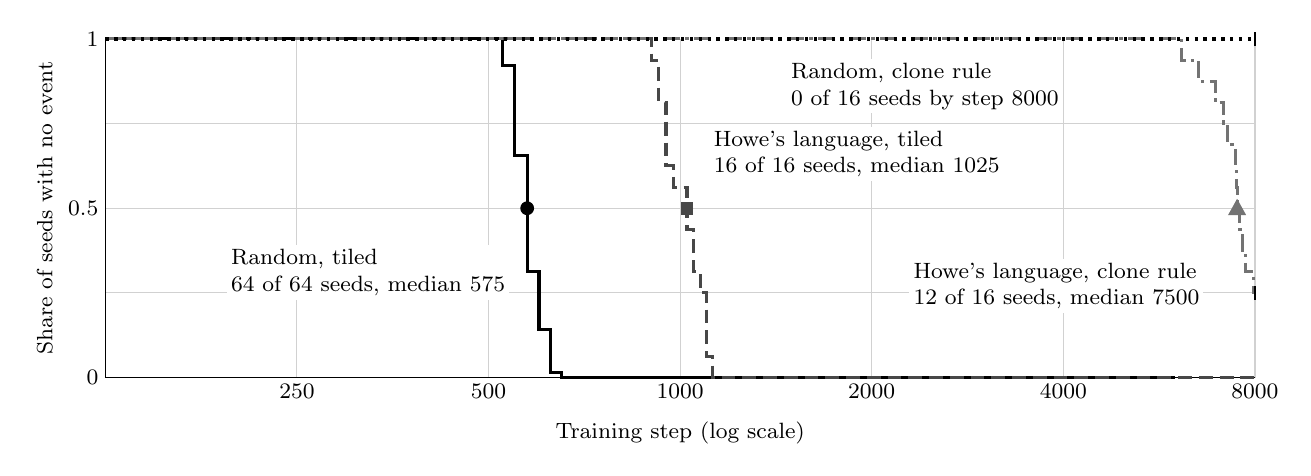
\begin{tikzpicture}
\draw[black!18, line width=0.4pt] (0.000,1.075) -- (14.600,1.075);
\draw[black!18, line width=0.4pt] (0.000,2.150) -- (14.600,2.150);
\draw[black!18, line width=0.4pt] (0.000,3.225) -- (14.600,3.225);
\draw[black!18, line width=0.4pt] (2.433,0.000) -- (2.433,4.300);
\node[anchor=north, inner sep=1.5pt, align=left, font=\footnotesize] at (2.433,-0.030) {250};
\draw[black!18, line width=0.4pt] (4.867,0.000) -- (4.867,4.300);
\node[anchor=north, inner sep=1.5pt, align=left, font=\footnotesize] at (4.867,-0.030) {500};
\draw[black!18, line width=0.4pt] (7.300,0.000) -- (7.300,4.300);
\node[anchor=north, inner sep=1.5pt, align=left, font=\footnotesize] at (7.300,-0.030) {1000};
\draw[black!18, line width=0.4pt] (9.733,0.000) -- (9.733,4.300);
\node[anchor=north, inner sep=1.5pt, align=left, font=\footnotesize] at (9.733,-0.030) {2000};
\draw[black!18, line width=0.4pt] (12.167,0.000) -- (12.167,4.300);
\node[anchor=north, inner sep=1.5pt, align=left, font=\footnotesize] at (12.167,-0.030) {4000};
\draw[black!18, line width=0.4pt] (14.600,0.000) -- (14.600,4.300);
\node[anchor=north, inner sep=1.5pt, align=left, font=\footnotesize] at (14.600,-0.030) {8000};
\draw[black, line width=0.5pt] (0.000,4.300) -- (0.000,0.000) -- (14.600,0.000);
\node[anchor=east, inner sep=1.5pt, align=left, font=\footnotesize] at (-0.030,0.000) {0};
\node[anchor=east, inner sep=1.5pt, align=left, font=\footnotesize] at (-0.030,2.150) {0.5};
\node[anchor=east, inner sep=1.5pt, align=left, font=\footnotesize] at (-0.030,4.300) {1};
\node[anchor=north, inner sep=1.5pt, align=left, font=\footnotesize] at (7.300,-0.500) {Training step (log scale)};
\node[rotate=90, anchor=south, font=\footnotesize] at (-0.55,2.150) {Share of seeds with no event};
\draw[black, line width=1.1pt] (0.000,4.300) -- (5.038,4.300) -- (5.038,4.233) -- (5.038,4.233) -- (5.038,4.166) -- (5.038,4.166) -- (5.038,4.098) -- (5.038,4.098) -- (5.038,4.031) -- (5.038,4.031) -- (5.038,3.964) -- (5.201,3.964) -- (5.201,3.897) -- (5.201,3.897) -- (5.201,3.830) -- (5.201,3.830) -- (5.201,3.762) -- (5.201,3.762) -- (5.201,3.695) -- (5.201,3.695) -- (5.201,3.628) -- (5.201,3.628) -- (5.201,3.561) -- (5.201,3.561) -- (5.201,3.494) -- (5.201,3.494) -- (5.201,3.427) -- (5.201,3.427) -- (5.201,3.359) -- (5.201,3.359) -- (5.201,3.292) -- (5.201,3.292) -- (5.201,3.225) -- (5.201,3.225) -- (5.201,3.158) -- (5.201,3.158) -- (5.201,3.091) -- (5.201,3.091) -- (5.201,3.023) -- (5.201,3.023) -- (5.201,2.956) -- (5.201,2.956) -- (5.201,2.889) -- (5.201,2.889) -- (5.201,2.822) -- (5.357,2.822) -- (5.357,2.755) -- (5.357,2.755) -- (5.357,2.688) -- (5.357,2.688) -- (5.357,2.620) -- (5.357,2.620) -- (5.357,2.553) -- (5.357,2.553) -- (5.357,2.486) -- (5.357,2.486) -- (5.357,2.419) -- (5.357,2.419) -- (5.357,2.352) -- (5.357,2.352) -- (5.357,2.284) -- (5.357,2.284) -- (5.357,2.217) -- (5.357,2.217) -- (5.357,2.150) -- (5.357,2.150) -- (5.357,2.083) -- (5.357,2.083) -- (5.357,2.016) -- (5.357,2.016) -- (5.357,1.948) -- (5.357,1.948) -- (5.357,1.881) -- (5.357,1.881) -- (5.357,1.814) -- (5.357,1.814) -- (5.357,1.747) -- (5.357,1.747) -- (5.357,1.680) -- (5.357,1.680) -- (5.357,1.612) -- (5.357,1.612) -- (5.357,1.545) -- (5.357,1.545) -- (5.357,1.478) -- (5.357,1.478) -- (5.357,1.411) -- (5.357,1.411) -- (5.357,1.344) -- (5.507,1.344) -- (5.507,1.277) -- (5.507,1.277) -- (5.507,1.209) -- (5.507,1.209) -- (5.507,1.142) -- (5.507,1.142) -- (5.507,1.075) -- (5.507,1.075) -- (5.507,1.008) -- (5.507,1.008) -- (5.507,0.941) -- (5.507,0.941) -- (5.507,0.873) -- (5.507,0.873) -- (5.507,0.806) -- (5.507,0.806) -- (5.507,0.739) -- (5.507,0.739) -- (5.507,0.672) -- (5.507,0.672) -- (5.507,0.605) -- (5.650,0.605) -- (5.650,0.537) -- (5.650,0.537) -- (5.650,0.470) -- (5.650,0.470) -- (5.650,0.403) -- (5.650,0.403) -- (5.650,0.336) -- (5.650,0.336) -- (5.650,0.269) -- (5.650,0.269) -- (5.650,0.202) -- (5.650,0.202) -- (5.650,0.134) -- (5.650,0.134) -- (5.650,0.067) -- (5.788,0.067) -- (5.788,0.000) -- (13.590,0.000);
\draw[black, fill=black, line width=0.7pt] (5.357,2.150) circle (0.075);
\draw[black!72, line width=1.1pt, dash pattern=on 5pt off 2.5pt] (0.000,4.300) -- (6.930,4.300) -- (6.930,4.031) -- (7.026,4.031) -- (7.026,3.762) -- (7.026,3.762) -- (7.026,3.494) -- (7.120,3.494) -- (7.120,3.225) -- (7.120,3.225) -- (7.120,2.956) -- (7.120,2.956) -- (7.120,2.688) -- (7.211,2.688) -- (7.211,2.419) -- (7.387,2.419) -- (7.387,2.150) -- (7.387,2.150) -- (7.387,1.881) -- (7.471,1.881) -- (7.471,1.612) -- (7.471,1.612) -- (7.471,1.344) -- (7.554,1.344) -- (7.554,1.075) -- (7.635,1.075) -- (7.635,0.806) -- (7.635,0.806) -- (7.635,0.537) -- (7.635,0.537) -- (7.635,0.269) -- (7.713,0.269) -- (7.713,0.000) -- (14.600,0.000);
\draw[black!72, fill=black!72, line width=0.7pt] (7.319,2.082) rectangle (7.455,2.218);
\draw[black!55, line width=1.1pt, dash pattern=on 6pt off 2pt on 1.2pt off 2pt] (0.000,4.300) -- (13.662,4.300) -- (13.662,4.031) -- (13.885,4.031) -- (13.885,3.762) -- (14.093,3.762) -- (14.093,3.494) -- (14.206,3.494) -- (14.206,3.225) -- (14.254,3.225) -- (14.254,2.956) -- (14.350,2.956) -- (14.350,2.688) -- (14.362,2.688) -- (14.362,2.419) -- (14.373,2.419) -- (14.373,2.150) -- (14.408,2.150) -- (14.408,1.881) -- (14.443,1.881) -- (14.443,1.612) -- (14.477,1.612) -- (14.477,1.344) -- (14.578,1.344) -- (14.578,1.075) -- (14.600,1.075);
\draw[black, line width=0.8pt] (14.600,0.985) -- (14.600,1.165);
\draw[black!55, fill=black!55, line width=0.7pt] (14.373,2.245) -- (14.278,2.074) -- (14.468,2.074) -- cycle;
\draw[black, line width=1.2pt, dash pattern=on 1.2pt off 2pt] (0.000,4.300) -- (14.600,4.300);
\draw[black, line width=0.8pt] (14.600,4.210) -- (14.600,4.390);
\node[anchor=east, inner sep=1.5pt, align=left, font=\footnotesize, fill=white] at (5.137,1.333) {Random, tiled\\64 of 64 seeds, median 575};
\node[anchor=west, inner sep=1.5pt, align=left, font=\footnotesize, fill=white] at (7.667,2.838) {Howe's language, tiled\\16 of 16 seeds, median 1025};
\node[anchor=east, inner sep=1.5pt, align=left, font=\footnotesize, fill=white] at (13.953,1.161) {Howe's language, clone rule\\12 of 16 seeds, median 7500};
\node[anchor=east, inner sep=1.5pt, align=left, font=\footnotesize, fill=white] at (12.167,3.698) {Random, clone rule\\0 of 16 seeds by step 8000};
\end{tikzpicture}
